\title{Изучение зарядово-обменных процессов \\ на установке СТРЕЛА}
\author{Новый экспериментальный подход к исследованию перезарядки на дейтроне}
\date{май~2012~г.}
\maketitle

\section{Введение}
В теории нуклон-нуклонного рассеяния, фундаментальное значение имеет извлечение
комплексных амплитуд матрицы рассеяния. Для получения всех амплитуд необходимо
проводить так называемый полный опыт, в результате которого должен быть получен
такой набор экспериментальных наблюдаемых, который позволяет провести
исчерпывающее описание процесса. Полный эксперимент включает в себя, в том числе
измерения с поляризованными частицами-снарядами, а также с поляризованными
мишенями. Это весьма большая и трудоёмкая задача.

Однако, в некоторых случаях возможно определить отдельные амплитуды матрицы
рассеяния, либо их совокупность, путём выбора некоторых экспериментальных
условий. Одной из возможностей является изучение реакции перезарядки на
дейтроне \dpchex с использованием неполяризованных протонов и неполяризованных
дейтронов, которая при некоторых условиях определяется только зависящими от
спина компонентами амплитуд. Появилась возможность оценить спин-зависящую часть
амплитуды \np рассеяния в рамках импульсного приближения, изучая
дифференциальное сечение этой реакции при малых передачах импульса. Эта идея
была предложена и формализована математически в целом ряде теоретических
работ~\cite{pom51,chew50,dean72_2}. Экспериментально такую серию работ пытались
решать в основном, в пучках сепарированных нейтронов от стриппинга ускоренных
дейтронов.

Целесообразным оказалось провести анализ экспериментальных данных, в которых
ускоренные дейтроны падали на протонную мишень. При такой постановке опыта
дейтроны монохроматичны, а вторичные два протона~--- продукты перезарядки
дейтрона на протоне, являются быстрыми и вылетают в переднем направлении под
малыми углами. Такой эксперимент был проведён на синхрофазотроне ЛВЭ ОИЯИ с
использованием в качестве одновременно детектора и мишени водородной пузырьковой
камеры. До начала наших исследований другие эксперименты с пучком дейтронов
практически отсутствовали.

На основе анализа экспериментальных данных было определено дифференциальное
сечение реакции перезарядки
$(d\sigma/dt)_{\dpchex}\,|\,_{t=0} = 30.2 \pm 4.1$~мб/(ГэВ/с)$^{2}$.
В пучке дейтронов получено отношение $R_{\np}$ дифференциальных сечений
перезарядки при $t=0$ в реакции \dpchex и \np. В рамках импульсного приближения
полученное значение $R_{\np} = 0.55\,\pm\,0.08$ свидетельствует о преобладающем
вкладе спин-зависящей части сечения \np рассеяния и согласуется с данными других
экспериментов в области близких энергий~\cite{mucha02,gla_mucha08}.

Изучение реакции перезарядки, проведённое с помощью камерной методики, позволило
предложить схему электронного эксперимента для изучения реакции перезарядки на
дейтроне в области энергий выше 1~ГэВ. В работе~\cite{glagolev96} было впервые
предложено исследование зарядово-обменных процессов в дейтрон-протонных
соударениях на ускорителе Нуклотрон с целью изучения спиновых эффектов в
неполяризованных пучках дейтронов с помощью электронной методики, для получения
статистически обеспеченного результата по определению вклада спин-зависящей
части амплитуды элементарного $np$-рассеяния.

Выбор конкретной геометрии эксперимента был выполнен на основе реальных событий
и расчётов методом генерации Монте"--~Карло с помощью программного пакета
GEANT3. Опираясь на данные по реакции $dp \rightarrow X$, полученные на
водородной пузырьковой камере, был промоделирован вариант эксперимента для
спектрометра, используя в качестве входных данных реальные события
$dp$-взаимодействий.  Для оценки фоновых условий были взяты все наблюдавшиеся
каналы реакций, информация о которых содержится на DST камерного
эксперимента. Фон от других реакций, кроме изучаемой реакции \dpfrag, которые
могли дать два положительно заряженных трека (например $dp \rightarrow
ppn\pi^{0}$) в направлении вперёд при ограниченной апертуре оказался
пренебрежимо малым~\cite{baz99}.

В результате моделирования была предложена схема установки
СТРЕЛА~\cite{strela_web}, электронного эксперимента для изучения реакции
перезарядки на дейтроне \dpchex с целью определения спин-зависящей части
амплитуды элементарной перезарядки \np. Были необходимы детекторы с хорошим
пространственным разрешением и быстрая современная электроника для считывания
большого потока информации. Не менее важной задачей был выбор системы отбора и
регистрации событий.

\section{Экспериментальная установка СТРЕЛА}
Установка представляет одноплечевой магнитный спектрометр, который расположен в
зале корпуса \textnumero205 ЛФВЭ ОИЯИ. Пучок дейтронов, выведенный из ускорителя
Нуклотрон, транспортируется и фокусируется магнитной оптикой канала ВП-1 на
мишень установки, которая находится в области перед фокусом Ф5,
рис.~\ref{fig:channel_VP1}.

\begin{figure}[h]
  \centering
  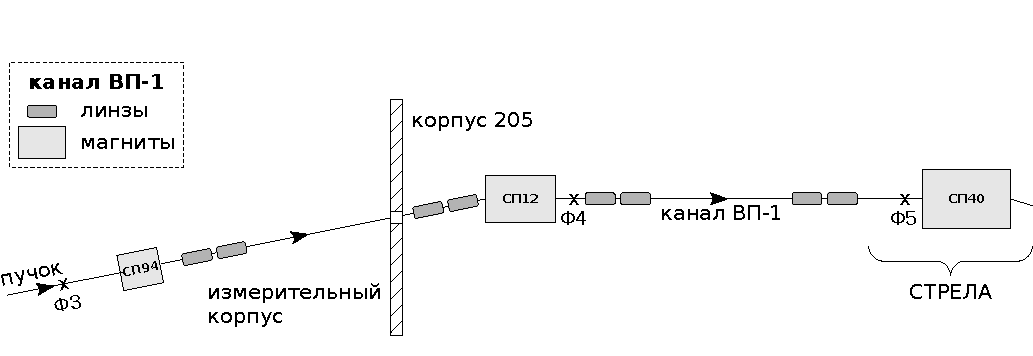
\includegraphics[width=1.00\textwidth]{channel_VP1.pdf}
  \caption{Канал ВП-1 выведенного пучка из ускорителя Нуклотрон с фокусами
    Ф3--Ф5. Транспортировка дейтронного пучка, до мишени установки СТРЕЛА,
    обеспечивается отклоняющими дипольными магнитами и фокусирующими
    квадрупольными линзами.}
  \label{fig:channel_VP1}
\end{figure}

\noindent
Основными элементами установки СТРЕЛА являются:
\begin{itemize}
\item блоки дрейфовых камер в качестве координатных детекторов,
\item электроника считывания информации,
\item сцинтилляционные счётчики используемые для запуска установки,
\item анализирующий магнит.
\end{itemize}

Для определения координат траекторий первичной и вторичных частиц в эксперименте
применяются дрейфовые камеры, которые объединяются в блоки. На
рис.~\ref{fig:strela_setup} приведена схема расположения всех блоков дрейфовых
камер, анализирующего магнита, мишени и сцинтилляционных (триггерных) счётчиков
на выведенном пучке дейтронов из ускорительного комплекса Нуклотрона.

\begin{figure}[h]
  \centering
  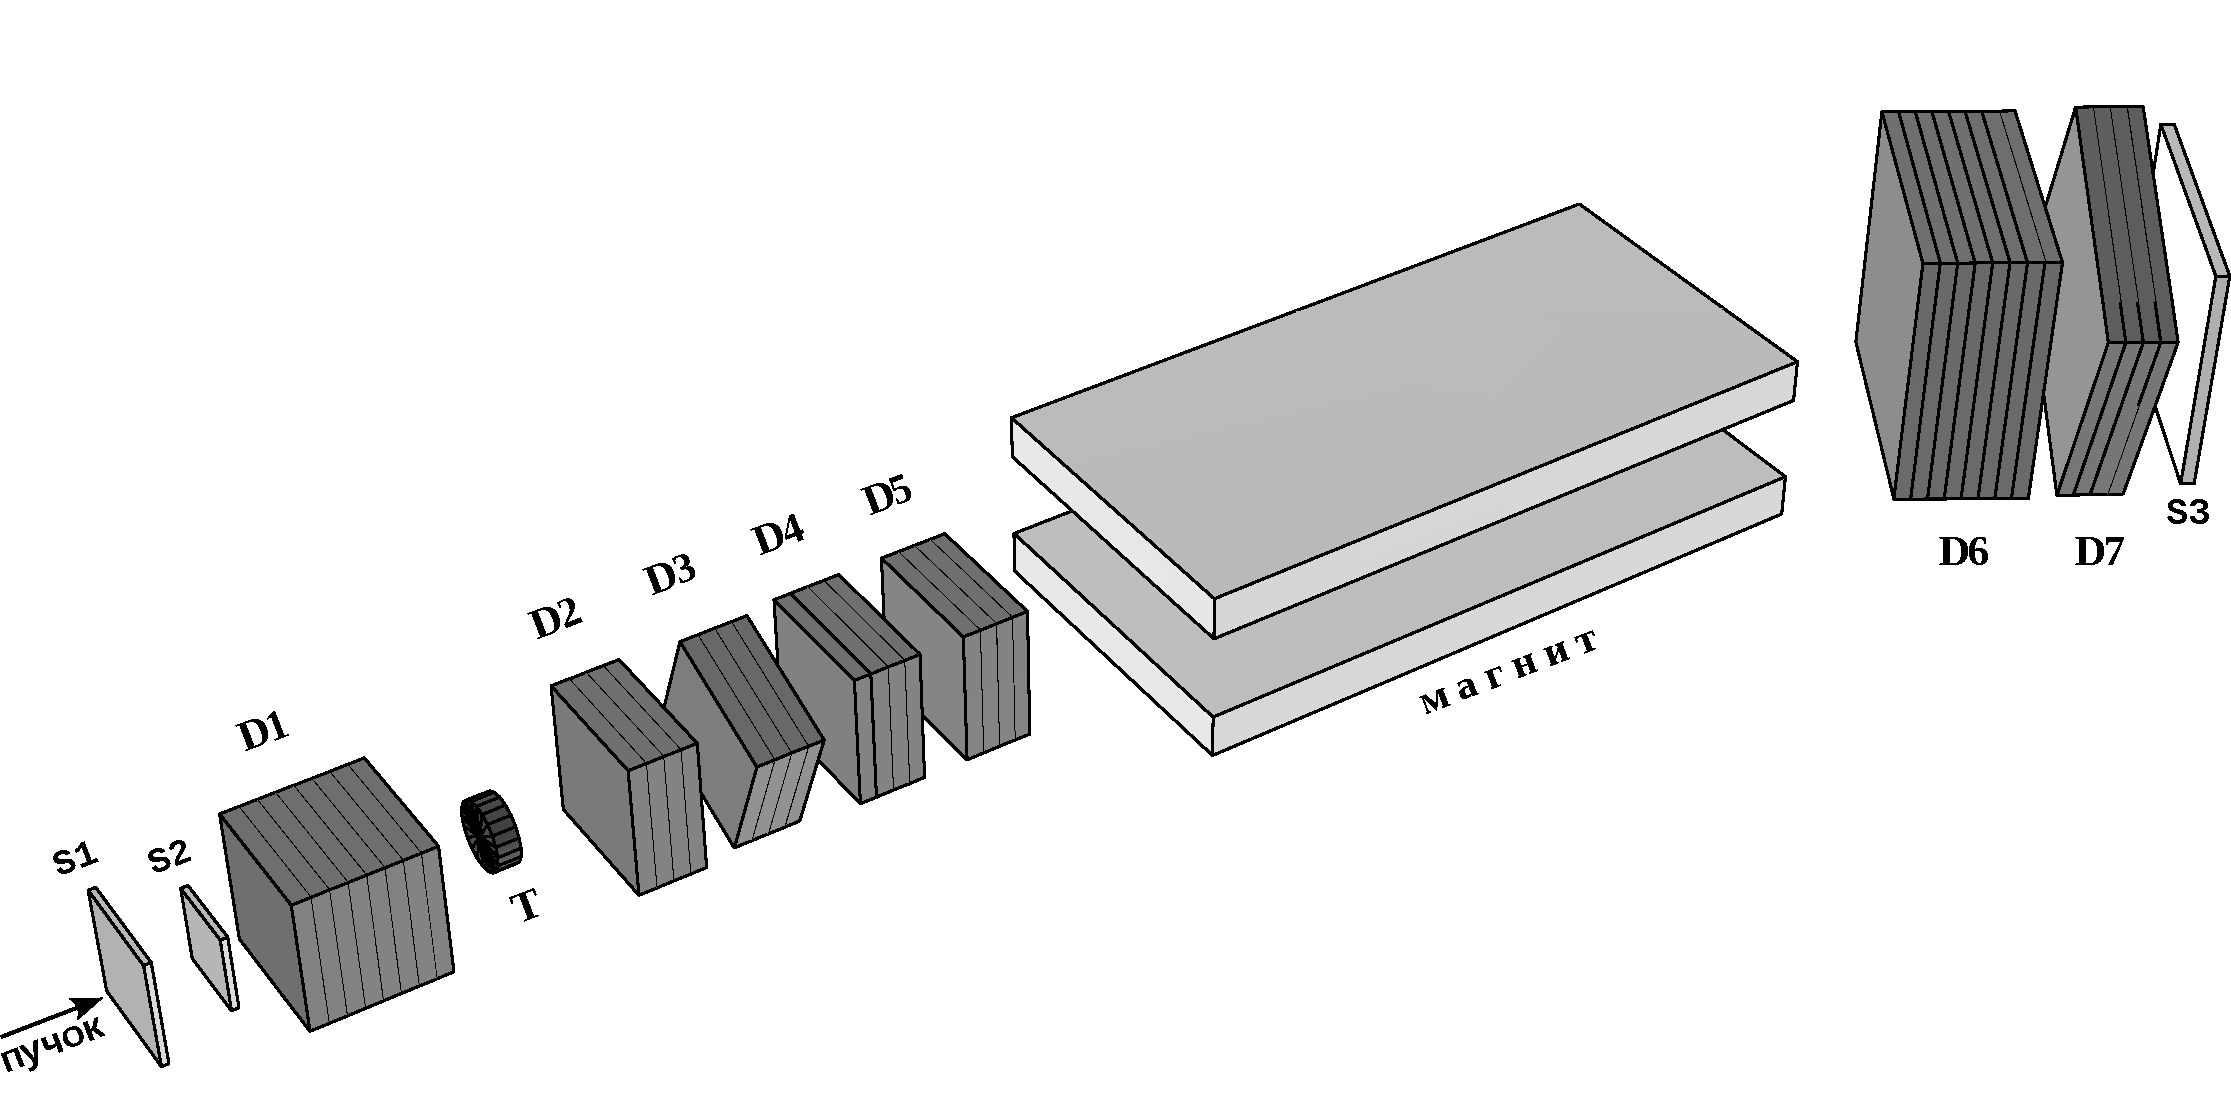
\includegraphics[width=1.00\textwidth]{strela_setup.pdf}
  \caption{Схема расположения дрейфовых камер и анализирующего магнита на
    экспериментальной установке СТРЕЛА. D1--D5~--- блоки <<маленьких>> дрейфовых
    камер с размером рабочей области 12.5~$\times$~12.5~см$^2$, D6--D7~---
    блоки <<больших>> камер с размером 25.0~$\times$~25.0~см$^2$, S1--S3~---
    сцинтилляционные счётчики,  Т~--- мишень.}
  \label{fig:strela_setup}
\end{figure}

В настоящее время используется 36 плоскостей дрейфовых камер, объединённых в 7
блоков. Каждый блок состоит из четырёх или восьми объединённых плоскостей
дрейфовых камер с различной ориентацией проволочек.

Длина дрейфового промежутка во всех камерах равна 21~мм.  Камеры в блоке
располагаются таким образом, что сигнальные проволочки в соседних плоскостях
сдвинуты относительно друг друга на 21~мм в направлении перпендикулярном оси
пучка. Такое расположение нитей позволяет устранить лево-правую неоднозначность
в определении пространственных координат треков частиц.

Координатная система дрейфовых камер выбрана следующим образом: ось $z$ для
блоков камер D1--D5 направлена по пучку падающих дейтронов, а для блоков камер
D6--D7, помещённых после магнита, по направлению максимума вылета протонов
стриппинга; оси $x$ и $y$ лежат в плоскостях камер так, что вместе с осью $z$
составляют правую тройку; координаты $u$ и $v$ используются для повёрнутых камер
вместо $x$ и $y$.

В таблице~\ref{tab:cham_config} приведена структура всех блоков дрейфовых камер
с их регистрируемыми координатами и количеством сигнальных проволочек в каждой
плоскости камеры, штриховая координата используется для сдвинутых проволочек.
\newcolumntype{M}{>{\columncolor[gray]{0.75}[0.90\tabcolsep]}c}
\begin{table}[h]
  \begin{center}
    \bigskip
    \resizebox{1.0\textwidth}{!} {
      \begin{tabular}{|l|c|c|c|c|c|c|c|c|c|c|c|c|c|c|c|c|}
        \hline
        Расположение блока & \multicolumn{16}{c|}{До мишени} \\
        \hline
        Блок & \multicolumn{4}{c|}{} &
        \multicolumn{8}{M|}{D1} & \multicolumn{4}{c|}{} \\
        \cline{6-13}
        Координата & \multicolumn{4}{c|}{} &
        $y$ & $y\,'$ & $y$ & $y\,'$ & $x$ & $x\,'$ & $x$ & $x\,'$ &
        \multicolumn{4}{c|}{} \\
        Число проволочек & \multicolumn{4}{c|}{} &
        4 & 3 & 4 & 3 & 4 & 3 & 4 & 3 & \multicolumn{4}{c|}{} \\
        \hline \hline

        Расположение блока & \multicolumn{16}{c|}{За мишенью} \\
        \hline
        Блок & \multicolumn{4}{M|}{D2} & \multicolumn{4}{M|}{D3} &
        \multicolumn{4}{M|}{D4} & \multicolumn{4}{M|}{D5} \\
        \cline{2-17}
        Координата & $y$ & $y\,'$ & $x$ & $x\,'$ & $u$ & $u\,'$ & $v$ & $v\,'$ &
        $x$ & $x$ & $x\,'$ & $x\,'$ & $y$ & $y\,'$ & $x$ & $x\,'$ \\
        Число проволочек &
        4 & 3 & 4 & 3 & 4 & 3 & 4 & 3 & 4 & 4 & 3 & 3 & 4 & 3 & 4 & 3 \\
        \hline \hline

        Расположение блока & \multicolumn{16}{c|}{За магнитом} \\
        \hline
        Блок & \multicolumn{2}{c|}{} & \multicolumn{8}{M|}{D6} &
        \multicolumn{4}{M|}{D7} & \multicolumn{2}{c|}{} \\
        \cline{4-15}
        Координата & \multicolumn{2}{c|}{} &
        $y$ & $y\,'$ & $y$ & $y\,'$ & $x$ & $x\,'$ & $x$ & $x\,'$ & $u$ & $u\,'$
        & $v$ & $v\,'$ &
        \multicolumn{2}{c|}{} \\
        Число проволочек & \multicolumn{2}{c|}{} &
        7 & 6 & 7 & 6 & 7 & 6 & 7 & 6 & 7 & 6 & 7 & 6 & \multicolumn{2}{c|}{} \\
        \hline
      \end{tabular}
    }
    \smallskip
    \caption{Конфигурация блоков дрейфовых камер на установке
      СТРЕЛА. $uv$-координаты повёрнутые относительно $xy$-координат вокруг оси
      $z$, штриховая координата означает сдвинутую плоскость камеры.}
    \label{tab:cham_config}
  \end{center}
\end{table}



%%% Local Variables:
%%% mode: latex
%%% TeX-master: "../strela2012"
%%% End:


До мишени располагается первый блок дрейфовых камер (D1) с размером рабочей
области 12.5~$\times$~12.5~см$^2$, имеющий четыре плоскости $y$-координат и
четыре плоскости $x$-координат. Первый блок служит для определения треков
пучковых дейтронов, падающих на мишень.

За мишенью располагаются четыре блока дрейфовых камер с такими же размерами
(<<маленькие>> камеры). Первый блок (D2) имеет две плоскости $y$-координат и две
плоскости $x$-координат, второй блок (D3)~--- две плоскости $u$-координат и две
плоскости $v$-координат. $uv$-координаты повёрнуты на 22.5$^{\,\circ}$
относительно $xy$-координат вокруг оси $z$, проходящей через центры блоков камер
в направлении падающего пучка. Далее следует блок дрейфовых камер (D4) с
четырьмя плоскостями $x$-координат, и последний блок (D5) имеет две плоскости
$y$-координат и две плоскости $x$-координат. Такой набор камер после мишени
позволяет надёжно идентифицировать два близко проходящих трека. Расстояние между
центрами двух крайних блоков D2 и D5 равно 65~см, между блоком D1 и блоком D2,
расположенными до и за мишенью, равно 90~см.

За анализирующим магнитом располагаются два блока дрейфовых камер с размерами
рабочей области 25.0~$\times$~25.0~см$^2$ (<<большие>> камеры). Ось $z$ данных
блоков (D6--D7) повёрнута на угол приблизительно~14$^{\,\circ}$ относительно оси
$z$ блоков камер (D1--D5), которые расположены перед отклоняющим магнитом.
Первый блок (D6) имеет четыре плоскости $y$-координат и четыре плоскости
$x$-координат, а второй блок (D7)~--- две плоскости $u$-координат и две
плоскости $v$-координат (повёрнутых также на 22.5$^{\,\circ}$ относительно
$xy$-координат). Расстояние между центрами блоков дрейфовых камер D6 и D7 равно
30~см.

Число всех регистрируемых сигналов с проволочек составляет 162. На каждой камере
установлены платы с микросхемами, в которых осуществляется усиление,
формирование и дискриминация входных сигналов от сигнальных проволочек дрейфовых
камер. Сформированные сигналы поступают на входы TDC модулей для оцифровки.
Полученная информация передаётся по оптической линии в персональный компьютер
для дальнейшей обработки.

На установке СТРЕЛА, для организации системы сбора экспериментальных данных
(DAQ), используются несколько модулей быстрой электроники в формате стандарта
VMEbus~\cite{vme85}. Данный стандарт предполагает создание
высокопроизводительных вычислительных систем модульного типа на основе
унифицированной магистрали. Он обладает достаточной универсальностью и
расширяемостью.

TDC модули (время-цифровые преобразователи) применяются для преобразования
(оцифровки) времени сформированных импульсных сигналов с дрейфовых камер. На
данный момент используются три TDC модуля. Один 64-канальный модуль (тип PhTDC)
и два 96-канальные модуля (тип TDC-96). Данные модули разработаны на базе
специализированной интегральной схемы HPTDC~\cite{hptdc04}. Это 32-канальный чип
время-цифрового преобразования с разрешением до 25 пс и оцифровкой обоих фронтов
импульсов.

Система запуска установки или отбора событий (триггерная система) должна
обеспечить набор событий реакции развала дейтрона при нулевом (близком к нулю)
угле рассеяния дейтрона на протоне. В нашем случае регистрируются два протона с
близкими импульсами из реакции перезарядки дейтрона на протоне \dpchex (развал
дейтрона с зарядовым обменом) и однопротонные события из реакции прямого развала
дейтрона \dpret. Запуск установки осуществлялся с помощью триггерных
счётчиков~--- три сцинтилляционных счётчика S1--S3
(рис.~\ref{fig:strela_setup}), которые определяют аксептанс установки и
вырабатывают сигнал для открытия временного окна регистрации сигналов с
дрейфовых камер и запуска системы сбора данных.

Установка СТРЕЛА была облучена в пучке дейтронов с импульсом 3.5~ГэВ/с. Система
стабилизации интенсивности выведенного пучка из ускорителя обеспечивает
равномерную интенсивность не ниже $\sim 10^{7}$ частиц в секунду. Так как
дрейфовые камеры могут работать при интенсивности не больше $\sim 10^{6}$ частиц
в секунду, то для уменьшения интенсивности использовался стальной коллиматор с
отверстием прямоугольной формы размером 4~$\times$ 4~мм$^2$ и длиной 1.2~м,
устанавливаемый в районе фокуса Ф3 после поворотного магнита СП-94 канала ВП-1
(рис.~\ref{fig:channel_VP1}). Применение коллиматора позволило при интенсивности
пучка в фокусе Ф3 на уровне $\sim 10^{7}$ частиц в секунду обеспечить
интенсивность пучка дейтронов на мишени установки в районе фокуса Ф5 на уровне
не больше~$\sim 5~\times 10^{5}$ частиц в секунду.

\begin{figure}[h]
  \centering
  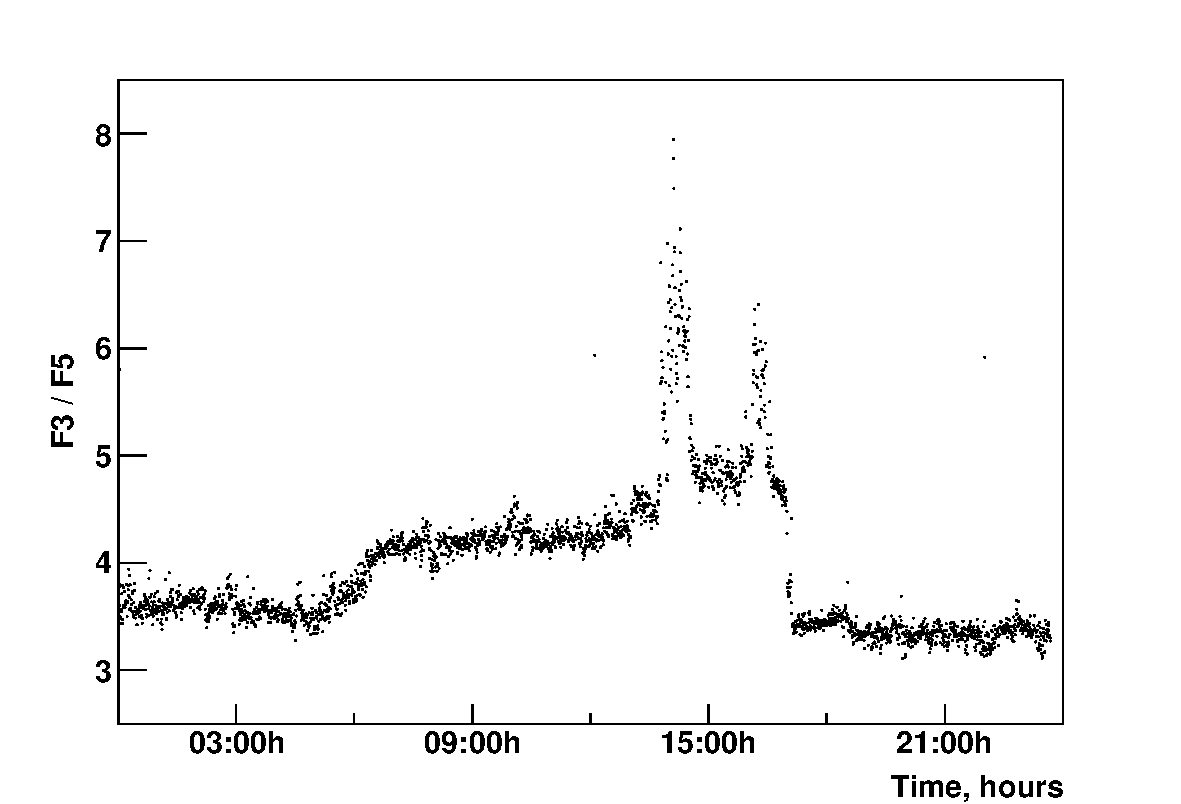
\includegraphics[width=0.65\textwidth]{beam_intensity.pdf}
  \caption{Изменение интенсивности выведенного дейтронного пучка на накале ВП-1
    в течение времени набора данных. Показано отношение счетов ионизационных
    камер, помещённых в фокусе Ф3 и Ф5 в зависимости от времени.}
  \label{fig:beam_intensity}
\end{figure}

Контроль интенсивности выведенного пучка осуществлялся с помощью ионизационных
камер. В процессе набора экспериментальных данных выявились нестабильности
выведенного пучка дейтронов. На рис.~\ref{fig:beam_intensity} приведено
отношение счетов с ионизационных камер расположенных в фокусах Ф3 и Ф5 в
зависимости от времени набора статистики. Повторные выбросы интенсивности пучка
приводили иногда к сбоям работы источников высоковольтного питания дрейфовых
камер. Использование коллиматора косвенно решает и задачу получения лучшей
временной структуры пучка.

\section{Время дрейфа}
Выбор дрейфовых камер в качестве координатных детекторов спектрометра обусловлен
возможностью получения высокого пространственного разрешения и более надёжного
отбора двух близко проходящих треков частиц. Изучение характеристик блоков
дрейфовых камер экспериментальной установки СТРЕЛА было проведено при облучении
полиэтиленовой мишени диаметром 5~см коллимированным пучком дейтронов с
импульсом 3.5~ГэВ/с на канале ВП-1 ускорительного комплекса Нуклотрона ЛФВЭ
ОИЯИ. Аппаратура установки облучалась в течение почти двух суток. В результате
облучения аппаратуры было набрано несколько миллионов триггеров для последующего
анализа.

Все блоки дрейфовых камер находятся в одном общем газовом объёме и продуваются
трёхкомпонентной газовой смесью аргона (72~$\%$), изобутана (25~$\%$) и
этилового спирта (3~$\%$), которая позволяет получить при напряжённости
электрического поля $\sim 1.5$~кВ/см режим постоянной скорости дрейфа
электронов и высокую линейную зависимость времени дрейфа от координаты трека
почти по всему объёму камеры. Замкнутая циркуляционная газовая система
обеспечивает продув каждого блока камер и выдерживает, с достаточной точностью,
стабильность газовых компонент в смеси. Средняя скорость потока смеси в системе
приблизительно 100~см$^{3}$/мин~\cite{filatova77}. С используемой
трёхкомпонентной смесью достигается стабильная работа камер и высокая
эффективность регистрации трековых частиц.

Применение дрейфовых камер требует нахождения соотношения между измеренным
временем дрейфа проходящей частицы и его преобразованием в расстояние
относительно данной сигнальной проволочки. Сначала используется <<интегральное>>
преобразование, после чего происходит поиск и реконструкция трека. Для получения
более корректного соотношения между временем дрейфа и расстоянием используется
итеративная процедура автокалибровки.

Временной спектр TDC одного из каналов показан на рис.~\ref{fig:tdc}.
Минимальное и максимальное время дрейфа ($T_{min},\,T_{max}$) для каждого канала
(проволочки) определяется аппроксимацией его временного спектра функцией
\begin{equation}
  \label{eq:tdc_fit}
  N(t) = p[2] + p[3]\,erfc\,\Biggl[\frac{(t - p[0])}{\sqrt{2}\,p[1]} \Biggr]\,,
\end{equation}
отдельно для минимального времени, $T_{min} = p[0] + p[1]$, и отдельно для
максимального, $T_{max} = p[0]$. $erfc(x)$~--- дополнительная функция
ошибок~\cite{erfc_web}. Параметры $p[2]$ и $p[3]$ можно использовать для
качественной проверки фита. Среднее полное время дрейфа составляет
$\sim$~450~нс.

\begin{figure}[h]
  \centering
  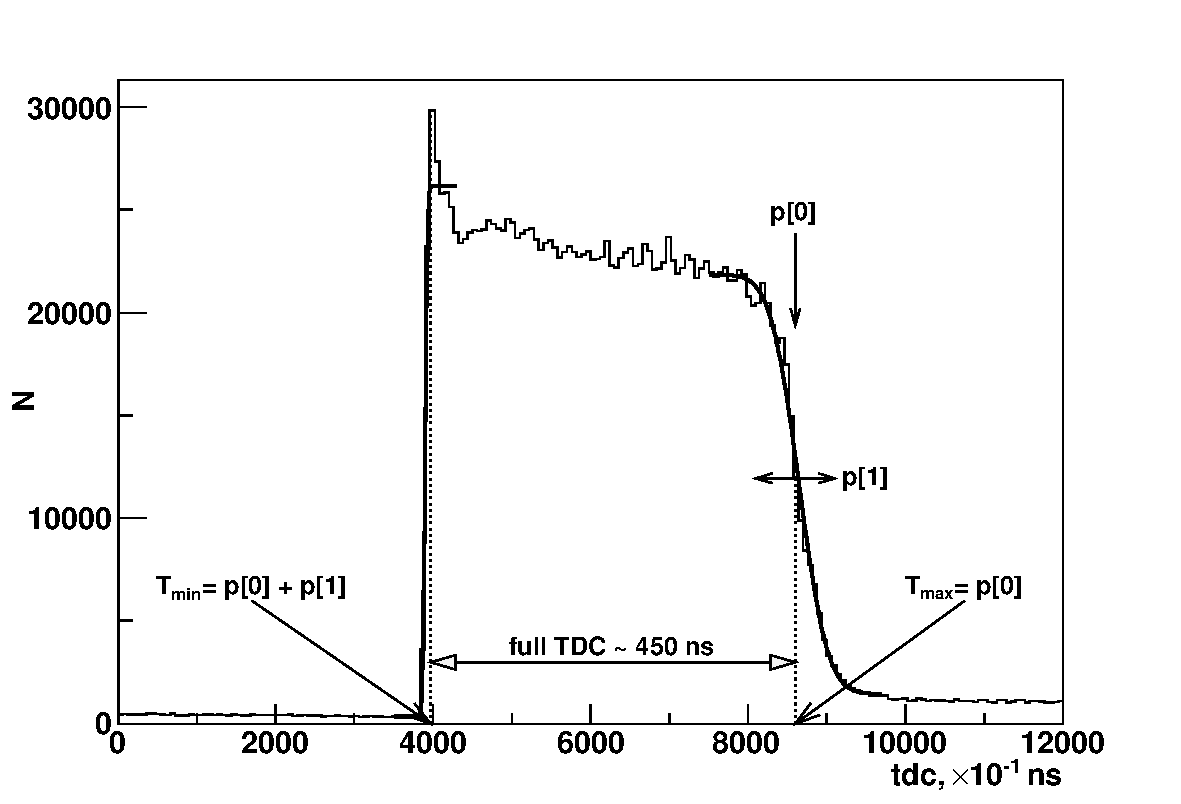
\includegraphics[width=0.65\textwidth]{tdc.pdf}
  \caption{Временной спектр $TDC$ одного из каналов (проволочек) дрейфовой
    камеры. Сплошные линии~--- аппроксимация распределения в области
    минимального $T_{min}$ и максимального $T_{max}$ времени
    функцией~\eqref{eq:tdc_fit}.}
  \label{fig:tdc}
\end{figure}

Соотношение между измеренным временем дрейфа и минимальным расстоянием между
анодной проволочкой и треком частицы имеет важнейшую роль при реконструкции
трека в дрейфовых камерах. Задача состоит в определении функции преобразования
времени дрейфа $t$ в расстояние $r$, так называемое $r(t)$-отношение, зависящее
от многих параметров: напряжённости электрического поля, состава газовой смеси,
давления, температуры, геометрии дрейфовой камеры~\cite{pesehonov86}.

Если предположить, что поток падающих частиц является равномерным, а
эффективность во всей области чувствительности проволочки постоянна, то скорость
дрейфа можно выразить как
\begin{equation}
  v_{d}(t) = \frac{dr}{dt} = \frac{dr}{dN}\,\frac{dN}{dt} =
  const\,\frac{dN}{dt}\,, \qquad
  const = \frac{dr}{dN} = \frac{R}{N_{tot}}\,,
\end{equation}
где $R$~--- длина дрейфового промежутка (21~мм), $N_{tot}$~--- полное число
событий и $dN/dt$~--- временное распределение (рис.~\ref{fig:tdc}).

Таким образом, функцию преобразования времени дрейфа $t$ в расстояние $r$ можно
выразить как
\begin{equation}
  r(t) = \int_{T_{min}}^{T_{max}} v_{d}(t')\,dt' = \frac{R}{N_{tot}}
  \int_{T_{min}}^{T_{max}} \frac{dN}{dt'}\,dt'\,.
\end{equation}
Заметим, что так полученное $r(t)$-отношение (рис.~\ref{fig:t2r}) будет
корректироваться (поправляться) в итеративном процессе
автокалибровки~\cite{gla_mucha10}.

\begin{figure}[h]
  \centering
  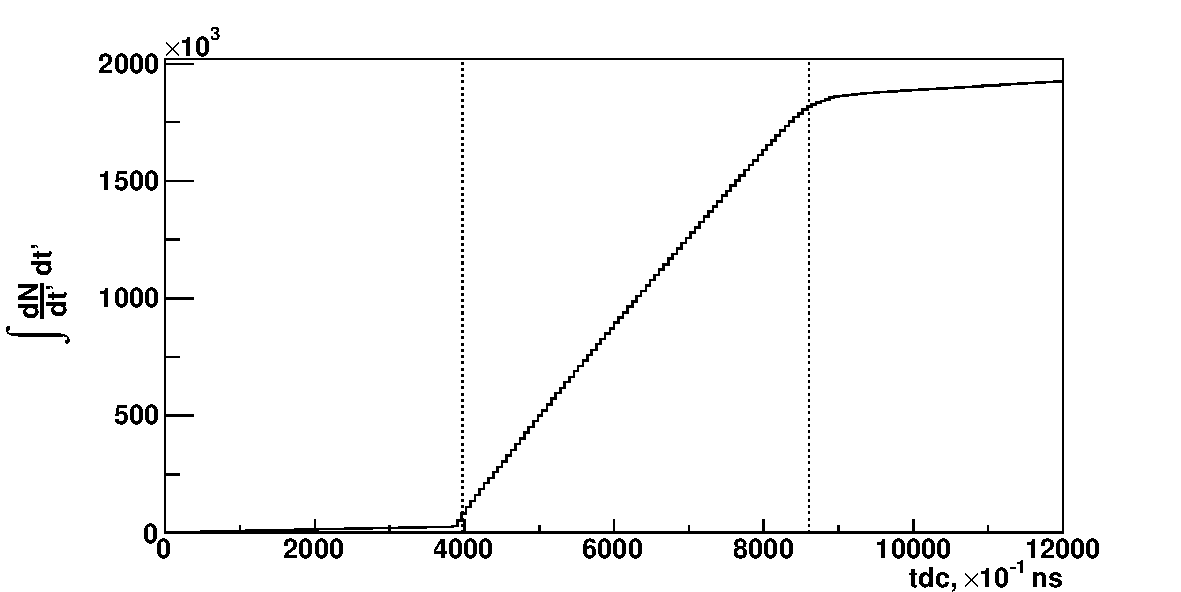
\includegraphics[width=0.49\textwidth]{t2r_t.pdf} \hfill
  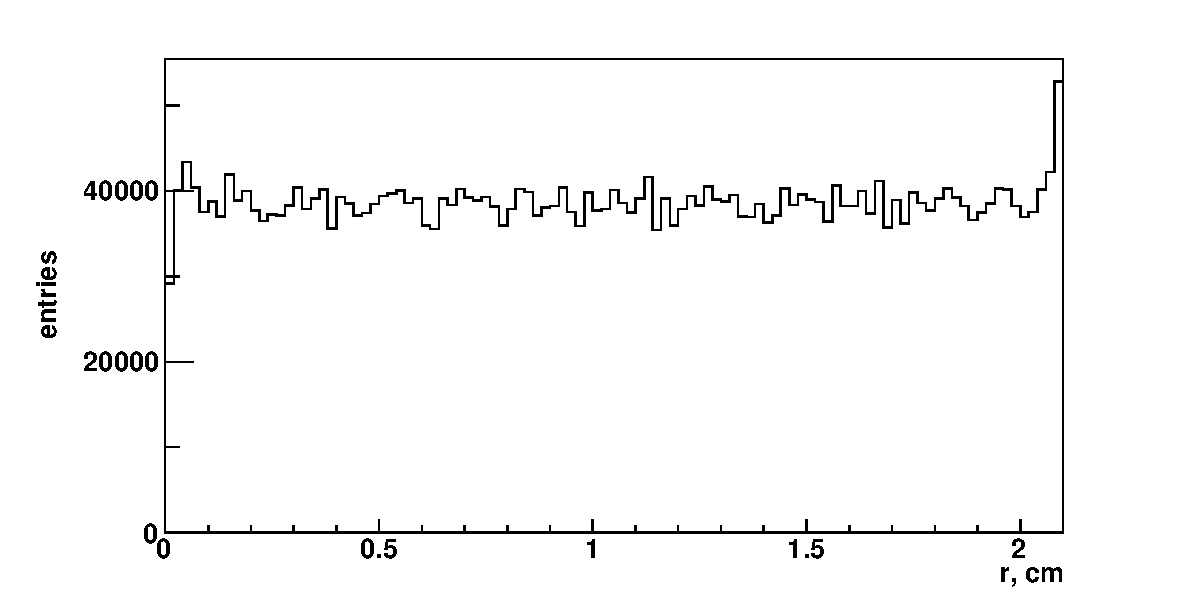
\includegraphics[width=0.49\textwidth]{t2r_r.pdf}
  \caption{На рисунке влево интегрированное время дрейфа $t$ проволочки из
    рис~\ref{fig:tdc}. Вправо~--- преобразованное расстояние $r$ между
    проволочкой и треком.}
  \label{fig:t2r}
\end{figure}

\section{Восстановление треков в дрейфовых камерах}
Поиск и реконструкция трека происходит отдельно для каждого блока
дрейфовых камер одной плоскости $xz$ или $yz$-координат. В зависимости от
конкретной задачи, можно программным путём, соединять (или разделять) блоки
камер в один мультиблок. В одном блоке (или мультиблоке) должно быть не менее
трёх слоев сигнальных проволочек, для возможности однозначного определения
трека. На рис.~\ref{fig:typo_2events} показан пример двух разных событий в одной
плоскости камеры, состоящей из четырёх слоёв проволочек.

\begin{figure}[h]
  \centering
  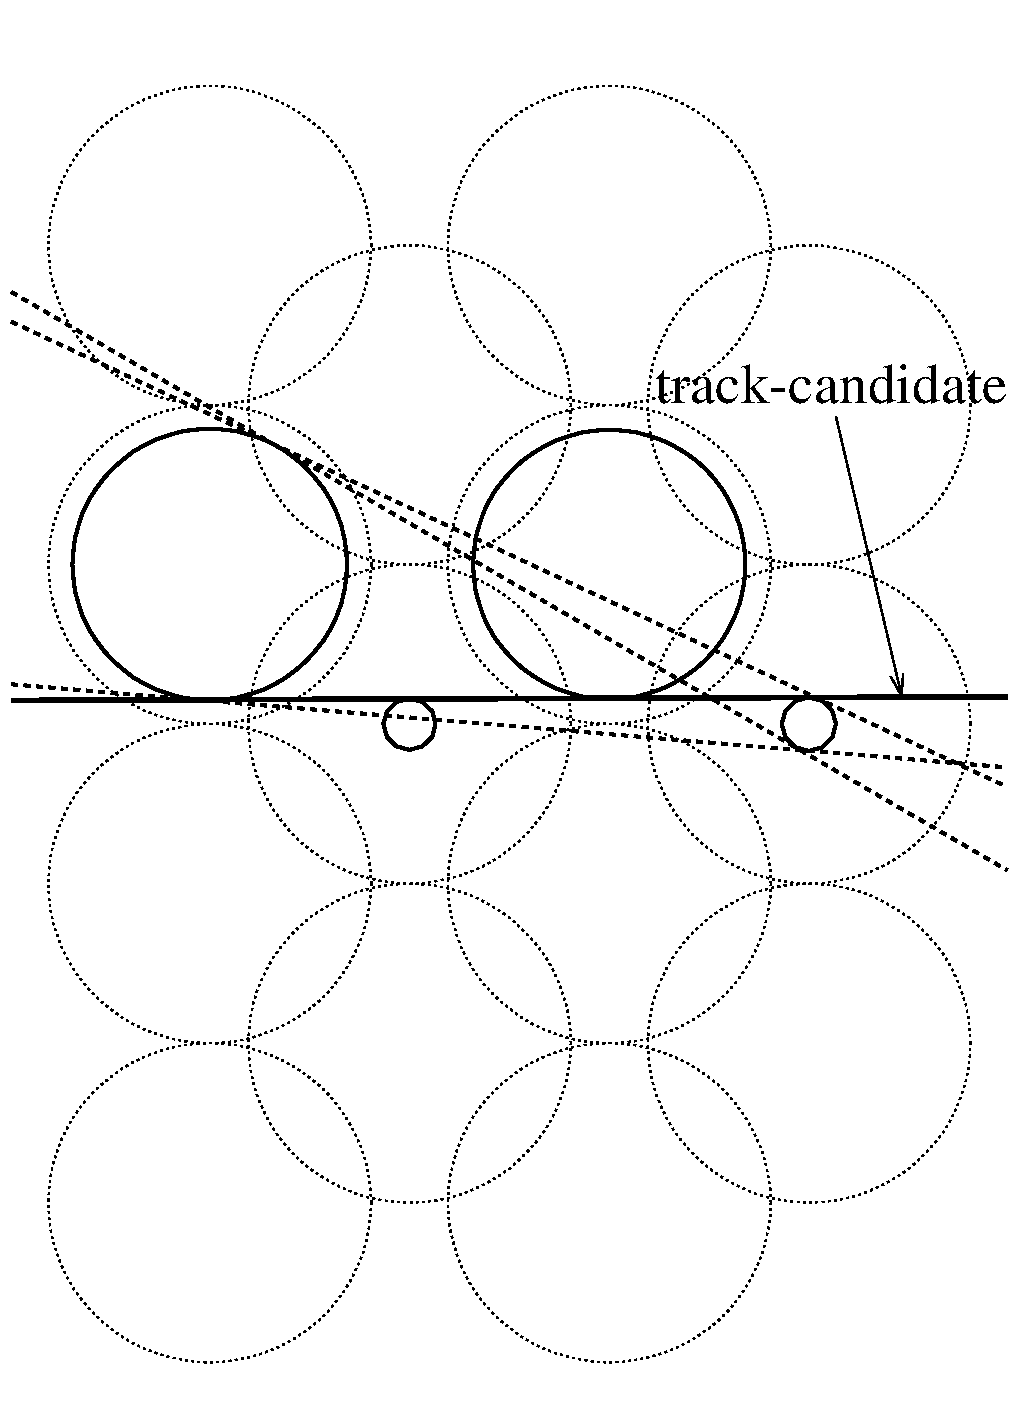
\includegraphics[width=0.41\textwidth]{event_112_run126.pdf} \hfill
  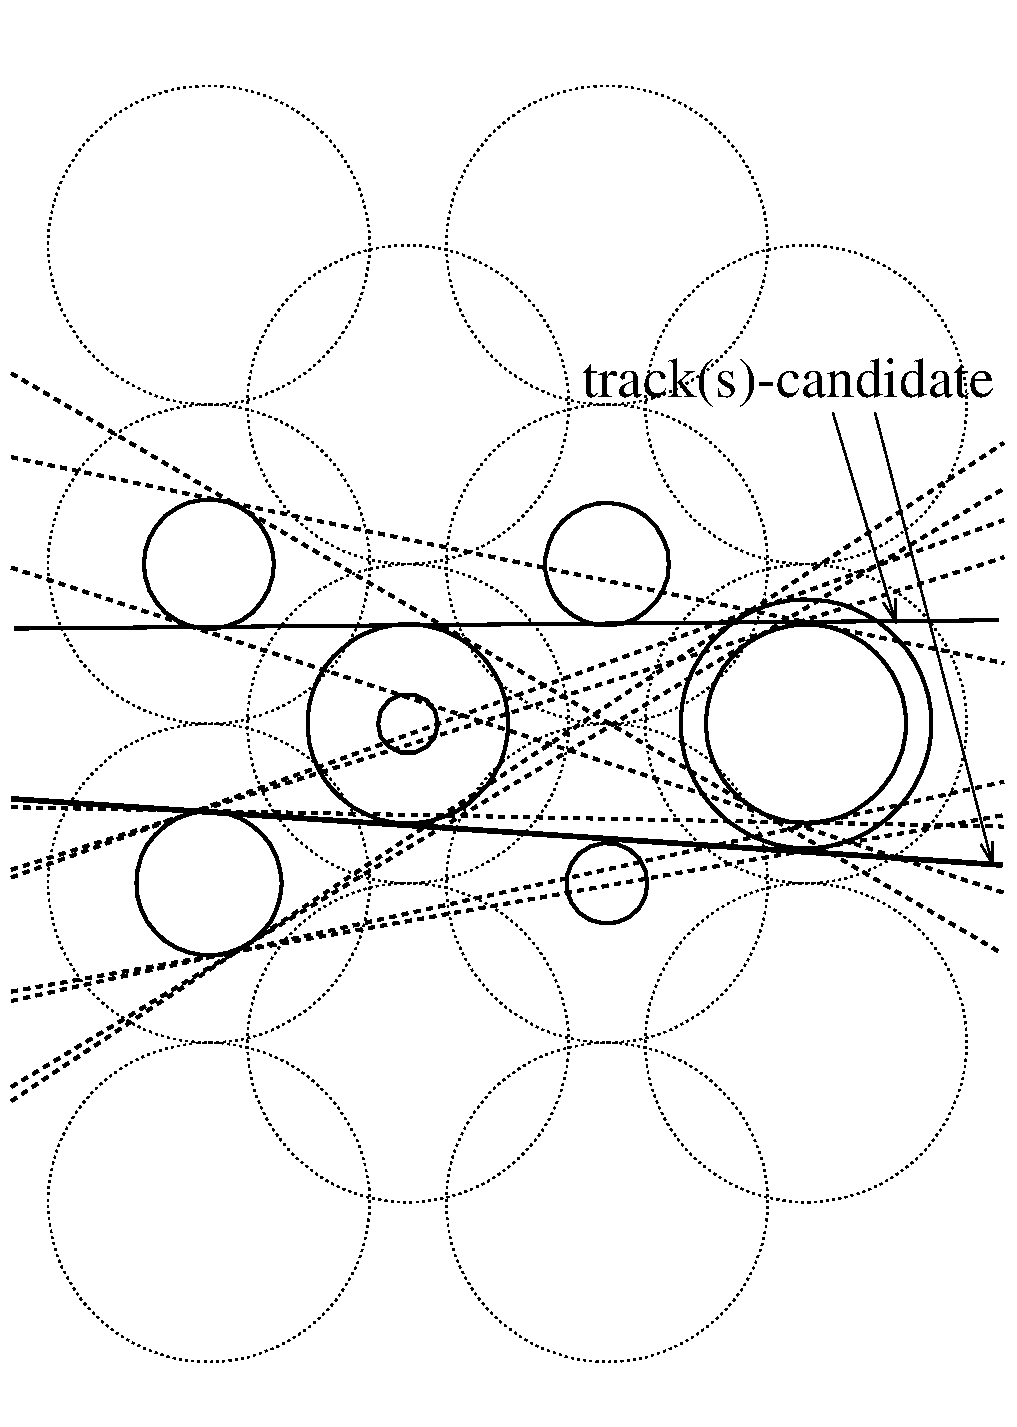
\includegraphics[width=0.41\textwidth]{event_104_run126.pdf}
  \caption{Пример проекции однотрекового (влево) и двухтрекового (вправо)
    события в одной плоскости блока первой дрейфовой камеры, состоящей из
    четырёх слоёв проволочек. Штриховые окружности представляют максимальную
    длину дрейфового промежутка, сплошные~--- расстояние трека от сигнальной
    нити. Для визуального изображения дрейфового промежутка используются
    окружности, центры которых проходят через сигнальные проволочки.}
  \label{fig:typo_2events}
\end{figure}

Последовательность поиска трека в упрощённом виде можно изложить следующим
образом:
\begin{enumerate}
\item Поиск пары сработавших проволочек из разных слоев камеры, имеющих
  наибольшее расстояние. Для пары окружностей, представляющих расстояние
  проекции трека от сигнальной нити, вычисляются параметры всех четырёх
  касательных, рис.~\ref{fig:typo_2events}.
\item Для каждой касательной вычисляется её расстояние $d$ от окружности
  сработавших проволочек. Если расстояние больше, чем заданное минимальное
  $d > d_{min}$, то сработавшая проволочка отбрасывается (не считается).
  $d_{min}$ обычно на порядок больше, чем пространственное разрешение камеры.
\item Если число сработавших проволочек $N_{hits}$ камеры, удовлетворяющих
  предыдущему условию, для касательной не менее заданного
  $N_{hits} \geq  N_{min}$, то касательная переходит в разряд кандидатов в трек.
  Для нашего примера (рис.~\ref{fig:typo_2events}) $N_{min}$ равно 4. Если
  кандидатов несколько, то оставляется тот, у которого сумма расстояний $d$
  минимальна.
\item Производится реконструкция трека и возвращение к 1.~пункту, т.е. поиску
  последующей пары в данном блоке дрейфовой камеры. Сработавшие проволочки,
  которые вошли  в восстановленный трек, не удаляются, и их можно использовать
  для поиска и реконструкции следующего трека.
\end{enumerate}

Трек-кандидат используется в процедуре реконструкции, восстановления
трека. Проекцию прямого трека в плоскости перпендикулярной к проволочкам блока
дрейфовой камеры можно параметризовать как уравнение прямой
\begin{equation}
  X = aZ + b
\end{equation}
с параметрами $a$ и $b$, рис.~\ref{fig:reco_scheme}.

\begin{figure}[h]
  \centering
  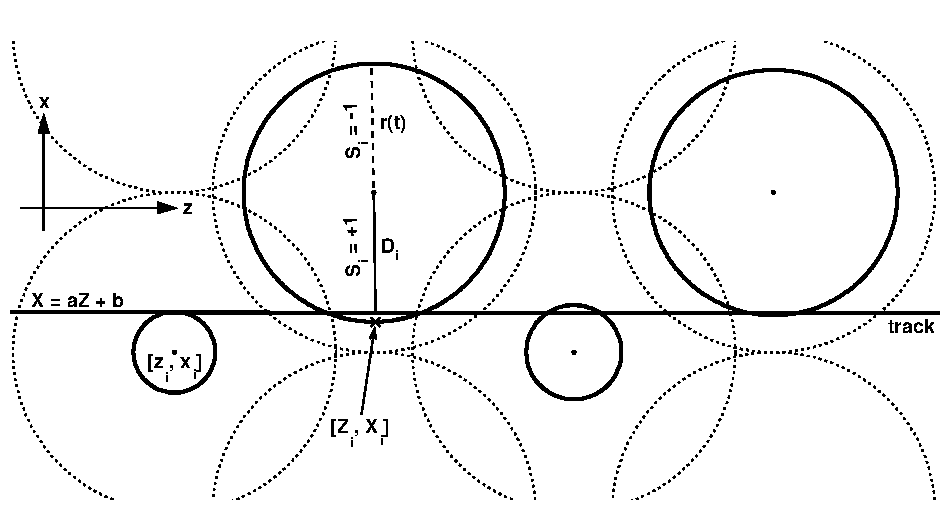
\includegraphics[width=0.75\textwidth]{event_137_run126.pdf}
  \caption{Определение параметров используемых при реконструкции трека в
    блоке дрейфовой камеры.}
  \label{fig:reco_scheme}
\end{figure}

Предположим, что трек имеет $N$ сработавших проволочек с координатами
$(z_i, x_i)$ для $i = 1, \ldots N$. Тогда расстояние между треком и $i$-й
проволочкой можно выразить как
\begin{equation}
  D_i = \frac{a z_i - x_i + b}{\sqrt{1 + a^{2}}}\,.
\end{equation}

Задача реконструкции трека состоит в получении параметров прямой $a$ и $b$
путём минимизации $\chi^2$-функции
\begin{equation}
  \label{eq:chi2_1}
  \chi^2 = \frac{1}{N-2}\sum_{i=1}^{N} [|D_i| -S_ir_i]^2 =
  \frac{1}{N-2}\sum_{i=1}^{N} \biggl[
  \Big|\frac{az_i - x_i + b}{\sqrt{1 + a^2}}\Big| - S_ir_i\biggr]^2\,,
\end{equation}
где $S_i$ имеет в зависимости от положения трека относительно проволочки
значение $\pm{1}$ (рис.~\ref{fig:reco_scheme}), $r_i$~--- расстояние между
треком и $i$-й проволочкой, полученное из функции преобразования времени дрейфа
$t$ в расстояние $r$. Величины параметров $a$ и $b$ получаем решением двух
дифференциальных уравнений
$\frac{\partial \chi^2}{\partial a} = 0$ и
$\frac{\partial \chi^2}{\partial b} = 0$, которые можно решить итеративно.
Уравнение~\eqref{eq:chi2_1} можно переписать следующим образом
\begin{equation}
  \label{eq:chi2_2}
  \chi^2 = \frac{1}{N-2}\sum_{i=1}^{N}
  \biggl[\frac{aZ_i - X_i + b}{\sqrt{1 + a^2}}\biggr]^2\,,
\end{equation}
где координаты проволочек $(z_i, x_i)$ заменяем координатами $(Z_i, X_i)$,
которые вычисляются как
\begin{equation}
  \label{eq:chi2_3}
  Z_i = z_i - S_ir_i \frac{a_0}{\sqrt{1 + a_0^2}}\,, \qquad
  X_i = x_i + S_ir_i \frac{1}{\sqrt{1 + a_0^2}}\,.
\end{equation}

Минимизируя $\chi^2$-функцию (уравнение~\eqref{eq:chi2_2}) методом наименьших
квадратов, получаем значения трековых параметров $a$ и $b$. Величину $a_0$ в
итеративном процессе последовательно заменяем новым значением $a$. В качестве
начального значение $a_0$ в уравнении \eqref{eq:chi2_3} используем параметр $a$
из трека-кандидата (касательной). Для частиц падающих на камеру под небольшими
углами можно принять $a_0 = 0$. В среднем, после двух--трёх итераций параметры
$a$ и $b$ практически не меняются, и если значение $\chi^2/ndf$ меньше
заданного, то трек считаем восстановленным.

\section{Автокалибровка}
Для реконструкции треков необходимо знать отношение между измеренным временем
дрейфа и его преобразованием в расстояние, поэтому получение правильного
$r(t)$-отношения, является одной из важнейших задач. Итеративную процедуру
определения $r(t)$-отношения с использованием трековой информации называем
автокалибровкой~\cite{bac97,pet05}.

Отметим, что $r(t)$-отношение, полученное в процессе равномерного облучения
частицами дрейфового промежутка не учитывает неравномерность напряжённости
электрического поля вдоль траектории дрейфа электронов, а это, в свою очередь,
приводит к изменению величины скорости дрейфа, и соответственно, к
дифференциальной нелинейности $r(t)$-отношения. Это возможно в конструкции
используемых дрейфовых камер, где напряжённость электрического поля вдоль
траектории дрейфа задаётся резистивной сборкой, резисторы которой имеет разброс
в несколько процентов.

Однако можно предположить приблизительно одинаковые условия в камере, для
которой выполняется автокалибровка. При необходимости можно программным путём
разделить камеры на меньшие или на группы проволочек, для которых предполагаем
те же самые условия. Иногда поиск и реконструкция трека происходит в одном
блоке (мультиблоке) камер, но процедура автокалибровки проделывается для
каждой камеры отдельно.

\begin{figure}[h]
  \centering
  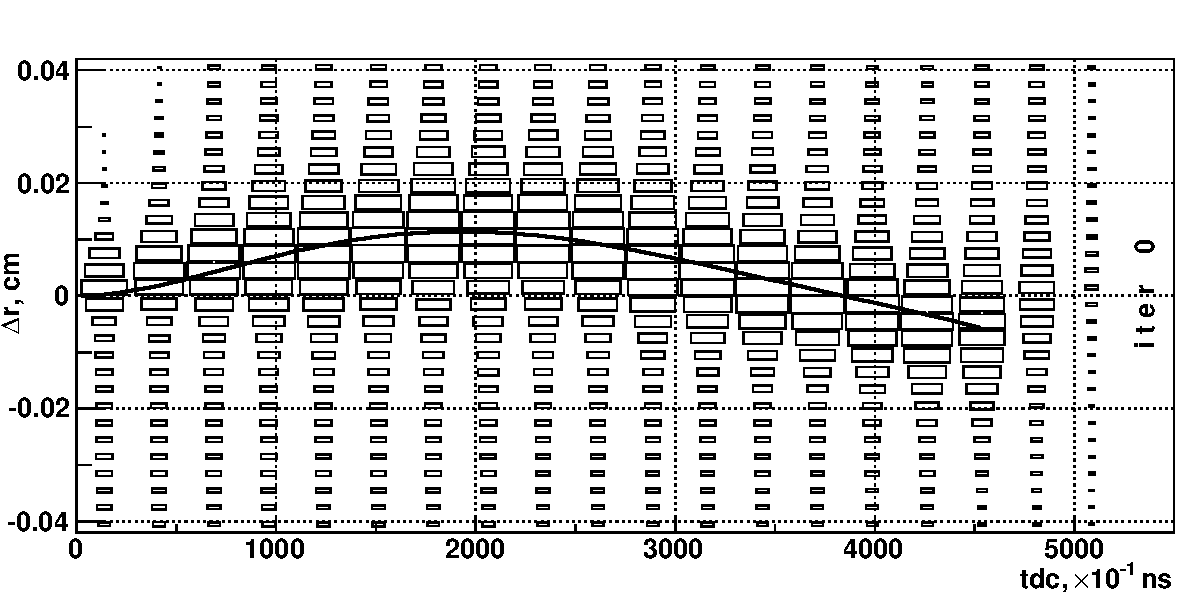
\includegraphics[width=0.65\textwidth]{multi_iter0.pdf}
  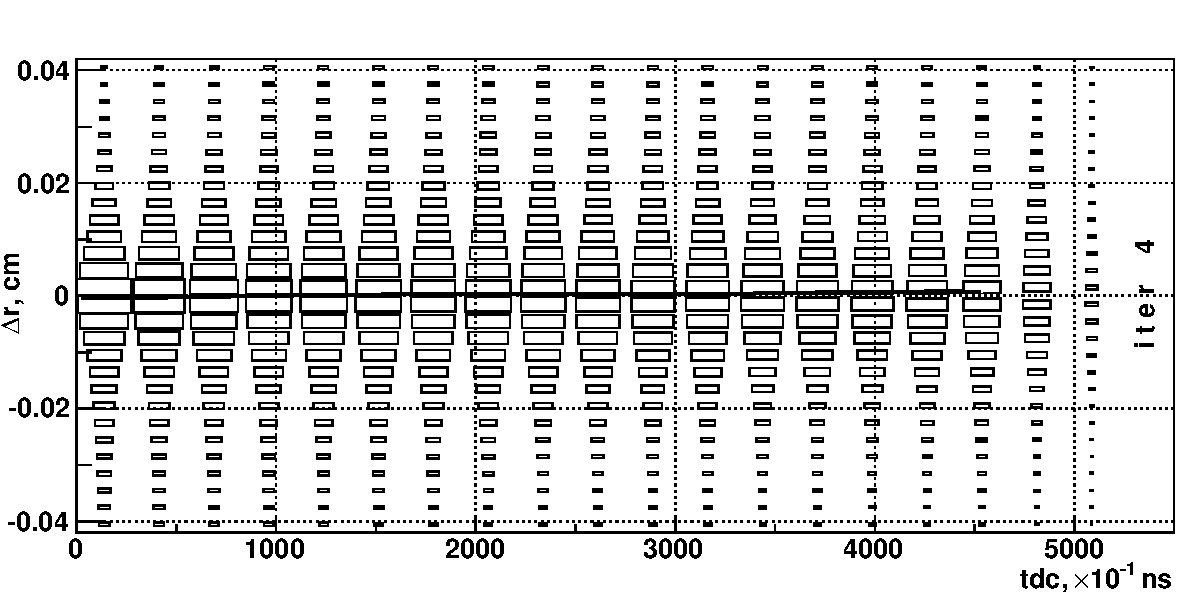
\includegraphics[width=0.65\textwidth]{multi_iter4.pdf}
  \caption{Зависимость распределения трекового остатка $\triangle r$ от времени
    дрейфа $t$ в одной плоскости блока больших дрейфовых камер. На верхнем
    рисунке исходное $r(t)$-отношения (интегральное преобразование времени
    в расстояние), нижний рисунок~--- после окончательной, четвёртой итерации
    автокалибровки. Размер прямоугольника пропорционален числу событий. Сплошная
    линия~--- аппроксимация средних значений трекового остатка для каждого
    временного интервала.}
  \label{fig:multi_iter}
\end{figure}

На рис.~\ref{fig:multi_iter} показана зависимость трекового остатка
$\triangle r$ (residual) от времени дрейфа в большой дрейфовой камере. Трековый
остаток можно определить как
\begin{equation}
  \triangle r = r - |D|\,,
\end{equation}
где $r$~--- расстояние полученное преобразованием ($r(t)$-отношение) времени
дрейфа $t$, а $D$~--- расстояние восстановленного трека от проволочки.

Распределение трекового остатка (его ширина) в основном определяется
пространственным разрешением дрейфовой камеры. Тем не менее, $\triangle r$
можно использовать при решении таких задач, как юстирование, сбалансирование
проволочек в блоках (мультиблоках) камер относительно друг друга или для
дополнительной оценки минимального и максимального времени дрейфа
($T_{min},\,T_{max}$). Ожидаемое среднее значение трекового остатка
$\triangle r \simeq 0$.

По горизонтальной оси двумерной зависимости распределения $\triangle r$ от $t$
(рис.~\ref{fig:multi_iter}) отложено время дрейфа с шагом гистограммы 27.5~нс.
Шаг выбран так, чтобы получить необходимое число временных интервалов. В нашем
примере оно равно 20. Для каждого временного интервала создаётся проекция
трекового остатка $\triangle r$. Полученные распределения остатков
аппроксимируются распределением Гаусса, среднее значение которого представляет
поправку $\delta_i$ к текущему $r(t)$-отношению в каждом $i$-м временном
интервале. Таким образом, получается новая, подправленная функция преобразования
времени дрейфа $t$ в расстояние $r$, с которой вновь выполняется реконструкция
трека.

В каждом следующем шаге процедуры автокалибровки $r(t)$-отно\-шение поправляется
в зависимости от предыдущей итерации. Поиск и реконструкция треков проводится
повторно до тех пор, пока значения поправок $\delta_i$ для всех временных
интервалов стабилизируются (приблизятся к нулевым значениям). В нашем примере
число итераций равно 4--5. Как меняется распределение трекового остатка в
зависимости от номера итерации, показано на рис.~\ref{fig:per_iterative}.
Видно, что с ростом номера итерации трековый остаток стремится к нулю, а ширина
распределения уменьшается.

\begin{figure}[h]
  \centering
  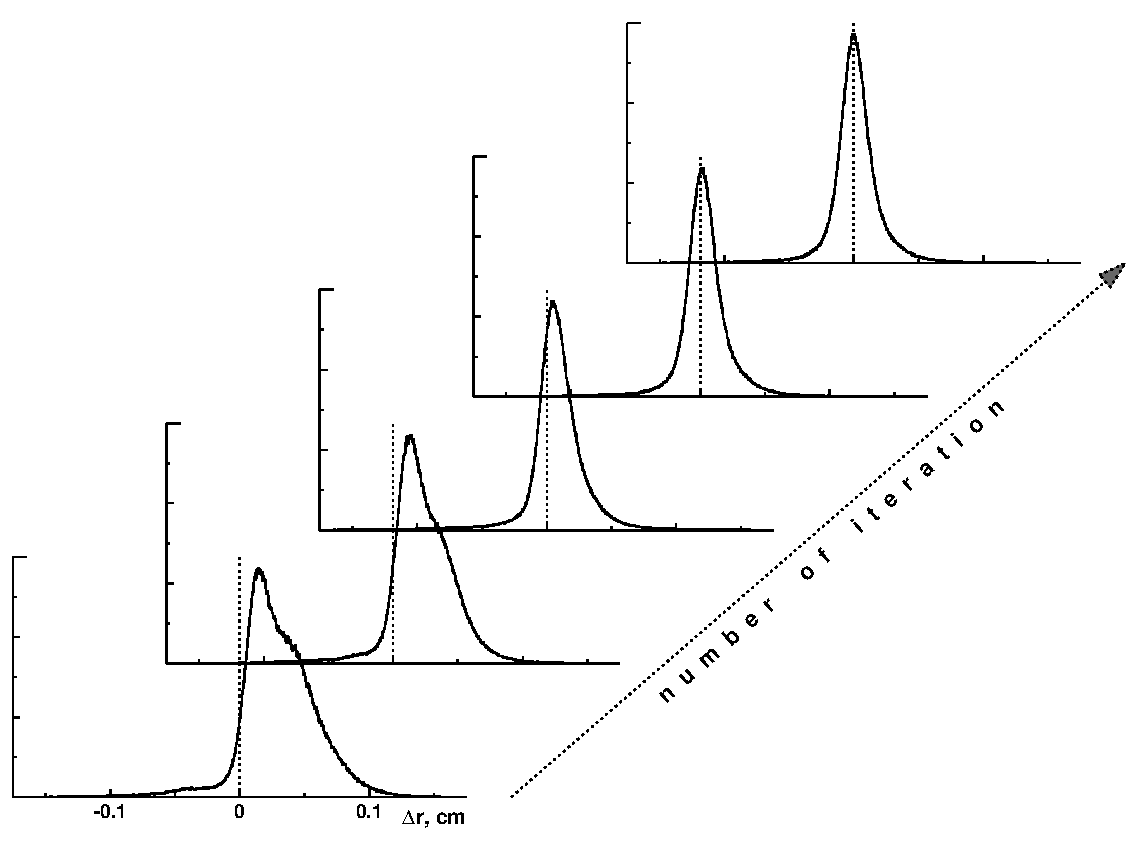
\includegraphics[width=1.00\textwidth]{c_per_iterative.pdf}
  \caption{Изменение распределения трекового остатка $\triangle r$ в зависимости
    от номера итерации в блоке больших дрейфовых камер.}
  \label{fig:per_iterative}
\end{figure}

Процесс автокалибровки выполняется только с однотрековыми событиями. Желательно,
чтобы угловой разброс треков в камере не превышал $\sim$~100~мрад. Если диапазон
наклонов треков, проходящих через камеру, большой, то итеративную процедуру
автокалибровки делаем отдельно для разных диапазонов углов наклона. Область
изменения угла наклона не должна превышать $\sim$~100--150~мрад.

Пространственное разрешение дрейфовой камеры определяется шириной распределения
трекового остатка данной камеры. Для вычисления разрешения $\sigma$
использовалась аппроксимация двойным распределением Гаусса,
рис.~\ref{fig:res_chambers}. Пространственное разрешение дрейфовых камер,
используемых на установке СТРЕЛА, лежит в диапазоне $\sim$~90--120~мкм.
Влиянием многократного рассеяния (дейтроны с импульсом 3.5 ГэВ/с) на разрешение
можно пренебречь.

\begin{figure}[h]
  \centering
  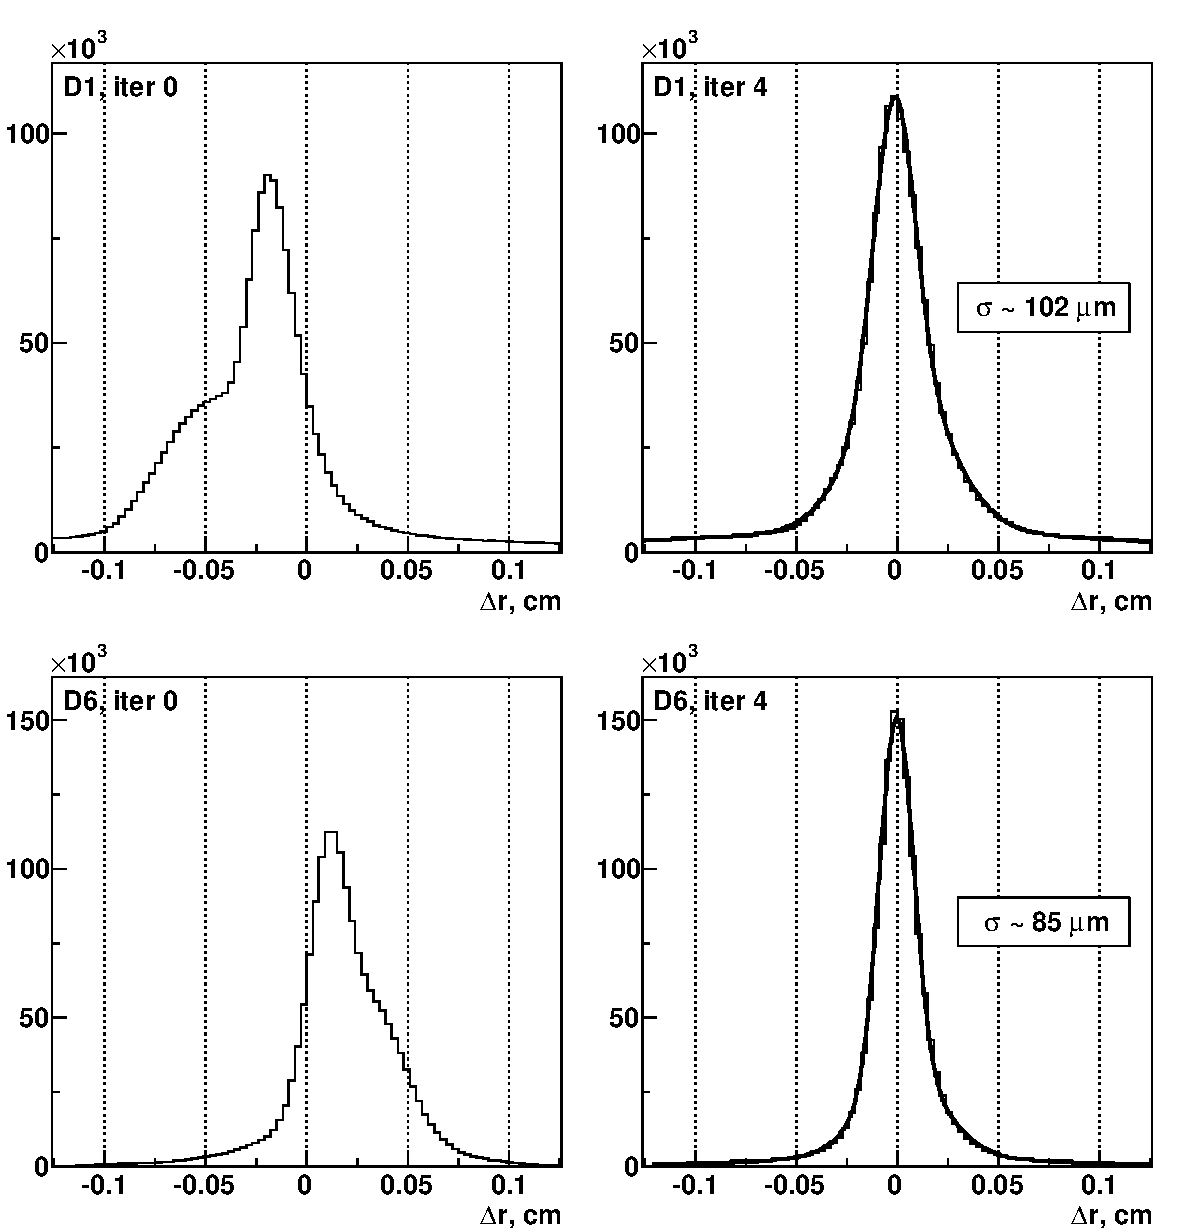
\includegraphics[width=0.85\textwidth]{res_chambers.pdf}
  \caption{Распределения трекового остатка $\triangle r$ в $xz$-плоскости
    дрейфовой камеры D1 и камеры D6. Слева~--- распределения с исходным
    интегральным $r(t)$-отношением, справа~--- после финальной четвёртой
    итерации автокалибровки, аппроксимированные двойным распределением Гаусса.}
  \label{fig:res_chambers}
\end{figure}

\section{Заключение}
На базе установки СТРЕЛА создан спектрометрический комплекс для изучения реакции
с обменом заряда в пучках дейтронов. Применение дрейфовых камер и их
пространственная разрешающая способность позволяют идентифицировать два протона
из реакции с обменом заряда на дейтроне. Полученные характеристики трековых
детекторов позволяют осуществить исследование зарядово-обменных процессов во
взаимодействиях дейтронов с протонами на установке СТРЕЛА. Описанная в работе
установка работает с 2007 года.



%%% Local Variables:
%%% mode: latex
%%% TeX-master: "strela2012"
%%% End:
